\chapter{GEOSX: A High-Performance Multiphysics Simulation Framework}
\chaptermark{Multiphysics Simulation Framework}
\label{ch:geosx_framework}

% ===================== SECTION =====================
\section{Introduction}
\label{sec:geosx_intro}

This chapter presents the overall design and several key components of a new multiphysics modeling framework targeting state-of-the-art and future massively parallel architectures, including upcoming exascale systems, called GEOSX \cite{geosx}, which is a collaborative effort between research groups from several institutions and companies \cite{geosx-website}.   We detail a few important contributions to the framework, including the development of compositional multiphase flow solver and linear algebra solver components, as well as describing the data structures and interfaces that form the foundation for the implementation of parallel multiscale preconditioner.

\subsection{Motivation and Design Goals}
\label{subsec:geosx_motivation}

Sustainable energy transition must rely heavily on a variety of subsurface energy systems, including  geological carbon storage (GCS) reservoirs, unconventional natural gas resources and geothermal systems.   A thorough understanding of the dynamic behavior of these systems is needed to predict and optimize their performance and ensure safety of operation.   Their behavior is driven by several tightly coupled physical processes, most notably porous media flow, transport, geomechanics and geochemistry, over a large range of spatiotemporal scales.   For example, when modeling injection into GCS deep saline reservoirs, accurate prediction of pressure buildup and associated mechanical deformation and stresses helps ensure the integrity of the cap rock and manage the risks of fault activation, CO\textsubscript{2} leakage and induced seismicity, while detailed modeling of fluid-rock interaction across and chemical reactions across scales improves our understanding of the interplay between CO\textsubscript{2} trapping mechanisms and storage capacity of these systems.

Unfortunately, in many pre-existing simulation tools coupling between different physical processes has often either been ignored or added as an afterthought, leading to loosely coupled models that may lack sufficient prediction accuracy.   For example, many commercial workflows involve transfer of information between a flow and a geomechanical simulator at predefined time intervals.   Incorporating new physics and tight coupling into a well established simulation package is an extremely challenging task, since it often requires fundamental changes in software architecture which are difficult to achieve while maintaining robustness, user familiarity and a plethora of supported features.   On the other hand, research simulators have been successful at implementing the necessary changes and prototyping and developing advanced physics, numerical models and coupling schemes \cite{Rin2017,Garipov2018}, but may lack robustness and performance required for large-scale modeling efforts due to a different set of goals and priorities (e.g. focusing on cutting-edge research).

At the same time, a fast-paced change in high-performance computing landscape has brought about new architectures (most notably, GPUs) with thousands of processing cores and orders-of-magnitude gains in raw compute power but also sophisticated memory hierarchies and programming models that additional require effort to take advantage of.   Updating legacy code to efficiently take advantage of parallelism on these platforms is often impossible or infeasible due to the amount and complexity of infrastructural changes involved and the need to redesign or outright replace many algorithms with their scalable versions.   In addition, as the architectures quickly evolve, changes made for one platform may become obsolete and non-portable.   A code that is designed for fine-grained parallelism from the ground up and built on top of a solid and portable parallel programming model can avoid both of these problems.

GEOSX is conceived and developed fundamentally as a novel massively parallel framework for fully coupled multiphysics subsurface simulation, aimed at taking advantage of current and next-generation high-performance computing architectures.   A specific set of design goals are:
\begin{itemize}
    \item Flexibility: support unstructured geologic grids with complex fault and fracture networks and wells, while solving combinations of coupled flow, transport, geomechanics and heat transfer problems.
    \item Modularity: developers see a highly modularized framework of components that are easy to add, while users interact with a unified simulator.
    \item Performance: striving to achieve near-peak performance on current and future architectures.
    \item Portability: while optimal algorithms and data structures are architecture-dependent, those differences are hidden behind portability abstractions.
\end{itemize}

\subsection{Framework Overview}
\label{subsec:geosx_overview}

GEOSX is developed in C++14 language standard, with additional Python interfaces and supporting modules.   Language extensions for CUDA (Compute Unified Device Architecture) and HIP (Heterogeneous Interface for Portability), the two major programming models for GPUs, are used when building the code on those platforms.   The framework has a modular architecture, consisting or a number of loosely coupled components that address various aspects of simulator workflow, such as data management, file I/O, discretization methods, constitutive models, linear algebra.   \Cref{fig:geosx_components} shows a simplified structure of core components of GEOSX.   All of these components ultimately are employed to build a collection of physics solvers that address specific (combinations of) physical processes.   Each physics solver acts as a driver for advancing a given set of solution and state variables to the next time level and makes use of an independent set of computational kernels (implemented as separate objects that manage their own data and execution) that may be customized and reused across solvers to facilitate the development of new fully implicit coupled solvers.   Execution of GEOSX is event-driven, with solver time stepping, visualization outputs, checkpointing and other tasks all invoked and coordinated in a consistent manner based on both a prescribed schedule of events and dynamic time step selection.   Next, we describe several core components of the framework, highlighting some of our contributions and describing in detail the key ingredients that enable the development of scalable parallel solvers and preconditioners.

\begin{figure} [htbp]
  \centerline{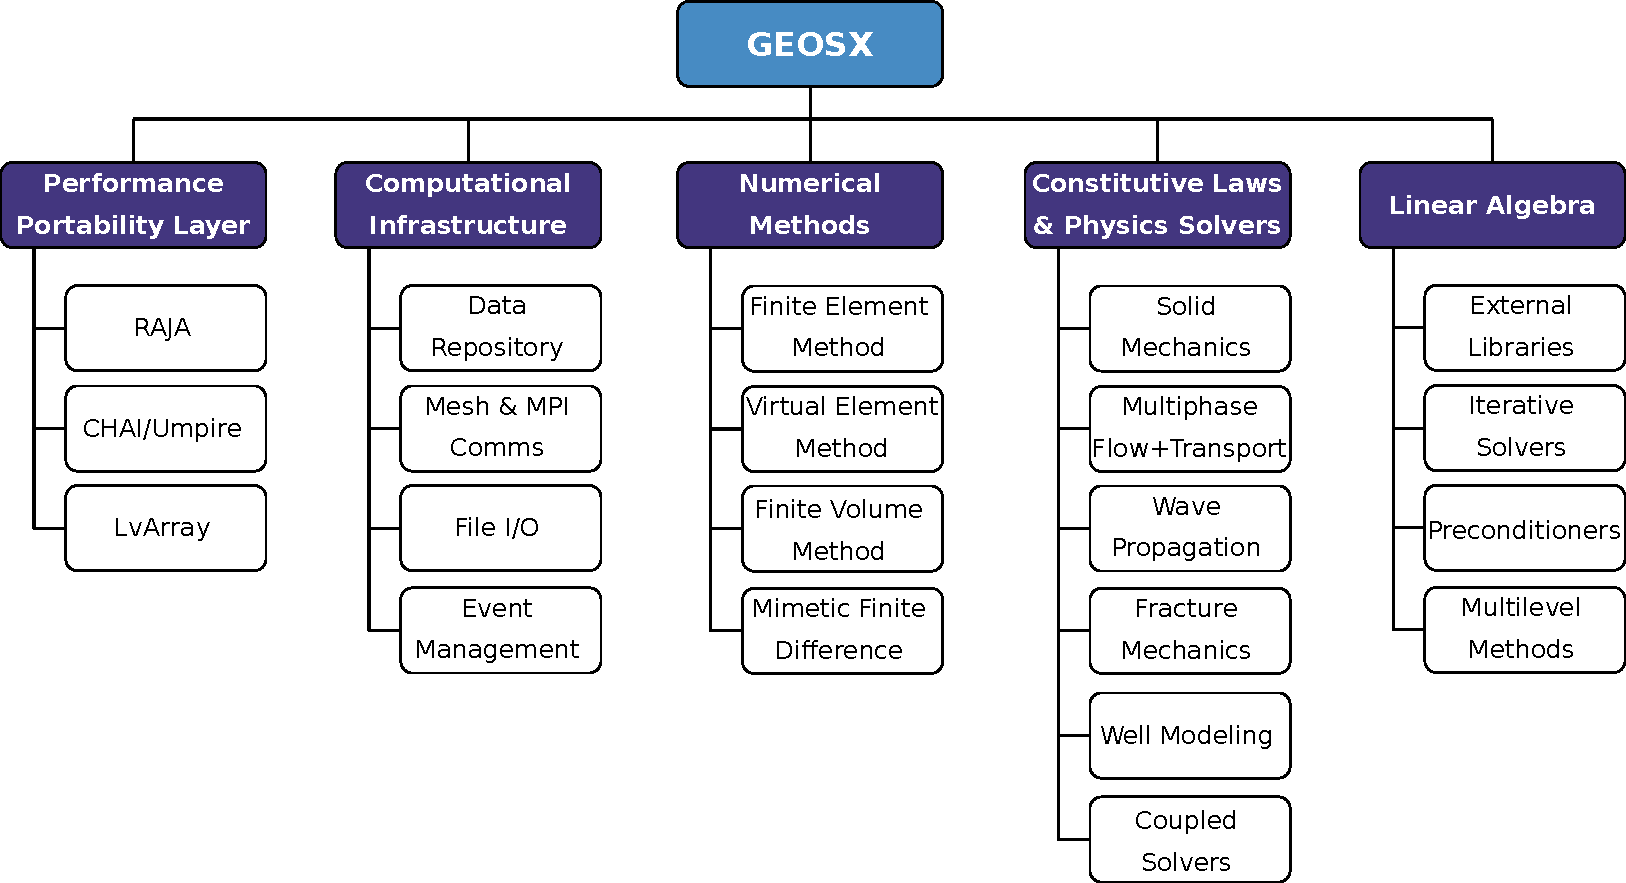
\includegraphics[width=0.9\linewidth]{figs/geosx}}
  \caption[Diagram of major GEOSX components]{\label{fig:geosx_components} A simplified diagram of GEOSX components, grouped into several logical groups}
\end{figure}

\section{Key Components}
\label{sec:geosx_components}

\subsection{Performance Portability Layer}
\label{subsec:geosx_components_portability}

Given the requirement for the framework to be forward-compatible with upcoming computing systems, our approach to leveraging parallelism is built on top of libraries that abstract away the details of particular hardware platform and vendor-specific application programming interfaces (APIs) and compiler instructions.   Most architectures provide two primary types of explicit resources --- compute and memory --- and both need to be dealt with in a portable way.   GEOSX is built on top of two separate types of abstractions provided by separate but interoperating libraries.

\subsubsection{Execution Model Abstractions}

Compute resource, or execution model, refers to decomposition and assignment of work over a number of execution units (multi-core CPU thread pools or blocks of GPU threads).   Execution abstraction used in GEOSX are available through RAJA library \cite{Beckingsale2019,raja}.   Loops over index spaces are the primary way of expressing independent work, and the library provides a \texttt{forall} pattern for writing parallel loops (also referred to as \textit{kernels}) as well as patterns for more complex control flow such as nested loops which allow for more flexible work partitioning.   The pattern accepts an execution \textit{policy} parameter, which specifies on which compute resource and how the loop is to be parallelized, along with an index space to iterate over and the work to be executed for each element in that space (the kernel \texttt{body}).   Under the hood RAJA takes care of decomposing work, mapping it to execution units and invoking a platform-specific API to initiate the computation according to the chosen policy.   The kernel body may be any function object callable with a single index argument, and often takes the form of a \texttt{closure} object (the result of a \texttt{lambda} expression that defines an anonymous function object in-place), which can conveniently carry arbitrary context necessary for the computation (such as views into arrays of physical quantities).   

In addition to kernel launching, RAJA contains portable abstractions over frequently used architecture-specific features such as atomic operations and block-shared memory on GPU (which falls back to regular memory on CPU targets).   Portable reductions are available in the form of objects that can be copy-captured in kernels and accumulate the final reduced value upon kernel exit.   Finally, more complex patterns that require dedicated implementations on different platforms (such as scan and sort) are also provided by the library.   With this set of primitives, large classes of numerical algorithms may be easily expressed in a portable way, and adapting the code to a new platform usually takes the form of using a different execution policy (as long as the necessary backend is implemented in RAJA).

\begin{figure} [htbp]
  \begin{subfigure}[t]{0.45\textwidth}
    \centering
    \begin{minted}[fontsize=\small]{cpp}
for (int i = 0; i < N; ++i)
{
    // kernel body
    c[i] = a[i] + b[i];
}
    \end{minted}
    \caption{\label{fig:raja_example_cpp} A simple C++ loop.}
  \end{subfigure}
  \hfill
  \begin{subfigure}[t]{0.45\textwidth}
    \centering
    \begin{minted}[fontsize=\small]{cpp}
RAJA::forall<Policy>(0, N, [=] (int i)
{ 
    // kernel body
    c[i] = a[i] + b[i]; 
});
    \end{minted}
    \caption{\label{fig:raja_example_raja} An equivalent RAJA loop.}
\end{subfigure}
\caption[RAJA loop example]{\label{fig:raja_example} Example of a C++ loop converted into a parallel RAJA loop. \texttt{Policy} may alias one of \texttt{loop\_exec}, \texttt{omp\_exec}, \texttt{cuda\_exec<num\_threads>}, etc. depending on target architecture.   Arrays \texttt{a}, \texttt{b} and \texttt{c} must be accessible in the chosen execution space.}
\end{figure}

\subsubsection{Memory Space Abstractions}

The second portability concern of a framework like GEOSX is dealing with multiple memory spaces.   Memory systems in parallel architectures like GPUs are heterogeneous, meaning system memory is physically and logically partitioned and some partitions (referred to as memory spaces) may not be accessible by all execution units.   Therefore any data accessed by a kernel must be first allocated in and copied to an appropriate memory space, and copies should only be performed when necessary (e.g. when data has been most recently modified in a different space) to avoid incurring extra cost.   This need is addressed by CHAI library \cite{chai} which provides convenient interfaces for tracking and managing memory allocations across different spaces.   CHAI itself is using Umpire library \cite{Beckingsale2020} containing a collection of memory-space aware allocators that abstract platform-specific memory management APIs.   CHAI coordinates with RAJA to infer a memory space appropriate for the compute resource of currently executing kernel and intelligently decide whether data must be copied into that space.   All simulation data containers (described next) in GEOSX are built on top of CHAI-managed memory buffers.

\subsection{Data Structures}
\label{subsec:geosx_components_data}

\subsubsection{High-performance Containers}

To support the RAJA-based kernel execution model and facilitate multiple-memory space semantics, GEOSX provides a number of specialized containers that are used across the code to store all mesh and simulation data, including solution and state variables, mesh connectivity maps, discretization information, variable-length model parameters, and any other data that must be accessed by kernels.   These containers, along with various some additional utilities for writing portable code are grouped into a separate library \texttt{LvArray}.
\begin{itemize}
    \item \texttt{Array} is a fundamental multidimensional array type, parametrized on data type, number of dimensions and memory layout.   The number of dimensions is static (compile-time), but array extents along each dimensions are specified at runtime.   The memory layout is chosen statically based on optimal memory access pattern on the target architecture.   For example, a coalesced read occurs on GPU when the kernel iteration parameter is used to index a unit-stride dimension of the array (typically dimension 0, corresponding to cell or node index of the mesh).
    \item \texttt{SortedArray} is a 1D array maintaining a sorted order and uniqueness of its elements, which makes it a fast and space-efficient representation of a \texttt{set} abstract type (known as a \texttt{flatset}). Quick $O(\log_2 n)$ lookup is provided via binary search, while element insertion is $O(n)$.
    \item \texttt{ArrayOfArrays} is a container representing a \textit{ragged} 2D array, i.e. one with variable-size second dimension.   All data is stored in a contiguous memory allocation, with offsets to keep track of the start of each sub-array.   This memory layout reduces the number of allocations and the amount of indirection needed for access, and corresponds to a widely used CSR (Compressed Sparse Row) storage format for sparse matrices.   In GEOSX it is most frequently used to represent connectivity graphs in mesh data structures.   New elements can be appended to any sub-array in a parallel kernel as long as sufficient capacity has been pre-allocated for it.   Moreover, elements can be appended to the same sub-array by concurrent threads using atomic instructions to increment sub-array size, which facilitates the use of multi-threaded kernels to build mesh maps.
    \item \texttt{ArrayOfSets} is similar to \texttt{ArrayOfArrays}, but also maintains uniqueness and sorted order of elements in each sub-array, similar to \texttt{SortedArray}.
    \item \texttt{CRSMatrix} is built on top of \texttt{ArrayOfSets} but stores both columns and entries, sorted by column index, while also providing an API for atomic operations on entries with fixed sparsity pattern.   It is used by all physics solvers to efficiently perform parallel assembly of implicit system matrices before handing it off to a linear solver.
\end{itemize}
By default, each of the above containers is backed by one or several CHAI-based linear memory buffer.   Each type also comes with a corresponding \texttt{View} type, which is a short-lived, non-owning data accessor that cannot reallocate (e.g. by resizing) the underlying container, but can invoke a data migration to another memory space when copied into a kernel execution context.   View types also control the data migration patterns: a \texttt{constant} view allows only read access and thus does not mark the data ''dirty'' (i.e. potentially modified) in the space in which it is used.   When used correctly, view types provide a transparent copy-hiding mechanism that is widely relied upon in GEOSX to perform operations across memory spaces.   As will be explained in \cref{ch:parallel_multiscale}, we have also built an efficient multilevel mesh data structure on top of these abstractions.

\subsubsection{Computational Grid}

GEOSX is designed from the ground up to support unstructured three-dimensional grids for modeling of a wide set of physics, and as such maintains an explicit representation and connectivity of all grid entities.   The grid is distributed across processes and each mesh object (cell, face, edge or node) is uniquely owned by one process, with possible ghosted representation on processes that own adjacent portions of the domain.   Each entity type is stored in an associated \texttt{Manager}, which provides useful services such as:
\begin{itemize}
    \item local-to-global (and inverse) mapping of object indices and ownership identification;
    \item management of associated data (registration, automatic sizing, (de-)serialization);
    \item synchronizing simulation data on ghosted objects (``halo exchanges``).
\end{itemize}
Each \texttt{Manager} also stores associated connectivity maps to other entities using the most efficient container, typically a 2D \texttt{Array} for fixed-size relations (e.g. each edge is connected to two nodes) or an \texttt{ArrayOfSets} for variable-sized ones (e.g. a node is connected to an arbitrary number of cells). 

Since GEOSX is designed for multiphysics simulations, the representation of elements has a more involved structure.   Elements of are grouped into \textit{regions} which allows for flexible mapping of physics and constitutive models to portions of the mesh (i.e. a solver may be assigned to a particular set of \textit{target} regions).   Each region type is specialized to a particular type of elements (e.g. 3D cells or 2D surfaces).   3D cell regions are further arranged into sub-regions by element shape (hexahedra, tetrahedra, etc.).    This allows us to use of memory-efficient data structures within each sub-region (2D arrays for face, edge and node maps).   Moreover, execution of finite-element kernels on GPU can be optimized, since for each sub-region key sizing parameters (number of nodes, quadrature points per element) can be made known at compile-time, through effective use of templates and static dispatching techniques, enabling loop unrolling and use of GPU registers.

\subsection{Constitutive Models}
\label{subsec:geosx_constitutive}

\subsubsection{Model Types}

GEOSX provides a large and extensible catalog of constitutive relations that describe various aspects of material (solid, fluid, etc.) behavior.   Models are grouped by their base type which defines model's interface in terms of input and output quantities.   Some of the commonly used model types (with examples of specific implementations):
\begin{itemize}
    \item solid deformation (elastic (transverse)isotropic/orthotropic, Drucker-Prager, Cam-Clay)
    \item single-phase fluid (slightly compressible)
    \item multiphase fluid (two-phase dead-oil, two- or three-phase black-oil, compositional EoS-based hydrocarbon, CO\textsubscript{2}-brine);
    \item porosity (constant, pressure-dependent, Biot)
    \item permeability (constant, Carman-Kozeny, parallel plates fracture)
    \item relative permeability (Brooks-Corey, Van Genuchten, Baker, table-based)
\end{itemize}
Each model implementation defines and can produce instances a companion \textit{compute} class (colloquially referred to as model's kernel \textit{wrapper}), that acts as a RAJA-friendly representation of the model that can be correctly copied into kernel execution contexts across memory spaces and used to perform computations.   In particular, a compute object contains inside of it memory-space aware \texttt{View}s into all relevant data, including model parameters and possible internal/history state (needed to implement hysteretic behavior).

\subsubsection{Constitutive Dispatch}

Since specific constitutive models are chosen by the user through input files, the framework needs a way to dispatch work to the right model during execution.   Traditional programming techniques for dealing with customizable behavior rely on dynamic dispatch, which usually takes the form of virtual functions or other similar types of indirect calls.   This works well when model computation across the entire grid points is \textit{batched} (i.e. all grid points are updated at once), but this forces the results to be committed to memory and prevents useful optimizations like kernel fusion (embedding the constitutive relation evaluation in another kernel, e.g. inside the finite-element assembly loop).   On the other hand, a point-wise compute interface is extremely flexible, but does not combine well with runtime dispatch:
\begin{itemize}
    \item on both CPU and GPU platforms, pointer indirection prevents code inlining and other forms of cross-function optimization;
    \item on GPU architectures, lack of compiler visibility into call targets also inhibits optimal register allocation, forcing suboptimal use of the register file and decreasing device occupancy.
\end{itemize}
To work around these issues, GEOSX relies on a form of \textit{static} (compile-time) dispatch, making effective use of C++ templates.   In essence, the technique consists of a template worker function parametrized on the actual type of model, and a runtime selector switch that checks the model type prior to kernel launch against a known set of derived models and dispatches to the appropriate instantiation of the worker.   In this scenario, the developer only writes one worker (kernel) function, and the compiler is forced to generates optimized code for each model type.   The downsides (increased build times and the need to modify the dispatch list upon adding a new model) are considered acceptable for the performance benefits gained.

\subsection{Physics Solvers}

Physics solvers are components of GEOSX that utilize all of the other modules and infrastructure to manage and advance simulation state ahead in time for a particular set of physical processes.   Some solvers describe a single physical phenomena (e.g. flow or deformation), while others manage coupled simulations and may dispatch work to two or more single-physics solvers as appropriate.   Each solver conforms to the same high-level interface which ensures interoperability, while internally may implement different numerical methods (for both time integration and spatial discretization), within some compatibility limits.   More specifically, each solver is responsible for:
\begin{itemize}
    \item registering relevant physical fields in the data repository;
    \item setting up and assembling implicit linear systems for Newton's method;
    \item setting up linear solver parameters and creating custom preconditioners if appropriate;
    \item updating primary and dependent fields and relevant constitutive models from an accepted solution, or resetting the time step in case of breakdown;
    \item calculating nonlinear residual norms;
    \item computing a requested time step size.
\end{itemize}
Most solvers act as drivers while delegating heavy computational work to a set of \textit{kernel} classes.   The benefit of this decomposition is that kernel classes can be customized and reused across several different physics solvers, facilitating code reuse.   The computational kernels are implemented using RAJA kernel launching mechanism and portable abstractions and data containers described in \cref{subsec:geosx_components_data}.   Most currently available physics solvers in GEOSX are thus fully GPU accelerated, meaning that they can perform the full simulation loop, including linear system assembly, entirely on device, without copying data back to host (unless necessary for file output), subject to GPU support in the selected linear algebra package.

\subsection{Compositional Multiphase Flow Solver}

We have designed and implemented a first-order finite-volume multi-component multiphase porous media flow and transport solver in GEOSX.   The solver provides modeling capabilities that power the key application areas of the framework, like geological carbon storage, unconventional reservoirs and many others.   In this section, we describe several important design decisions and implementation details that allow for efficiently executing the solver kernels on both CPU and GPU platforms.

\subsubsection{Nonlinear Formulation}

As is common in reservoir simulation practice, the conservation equations are implemented in the most general form \cref{eq:mass_balance_mp}, allowing for an arbitrary number of components to be partitioned into an arbitrary (though typically small) number of fluid phases.   The choice and labeling of components and phases is left to the user, who must choose one of a catalog of fluid models that are developed and maintained independently of the solver, and range from immiscible two-phase to specialized CO\textsubscript{2}-brine, to general equation-of-state based hydrocarbon mixtures.

An important design decision is the choice of nonlinear formulation, which refers to the choice of solution variables as well as a specific form of nonlinear equations to be solved via Newton's method.   Pressure of one (reference) phase is almost always used as an independent variable.   There are two commonly used choices for the transport part \cite{Cao2002}:
\begin{itemize}
    \item \textit{natural} formulation employs (a subset of) saturations $S^\alpha$ and phase compositions $y_i^\alpha$ as independent variables --- the specific choice depends on phase state of each cell (i.e. which phases are present at given conditions);
    \item \textit{overall} formulation (sometimes referred to as \textit{global}) uses a set of composition variables that are globally defined without being intrinsic to a particular phase, such as overall component fractions $z_i$ (mole fraction of component $i$ in the system) or partial densities $\rho_i$ (total mass or moles of component $i$ divided by total fluid volume).
\end{itemize}
Natural formulation historically has been preferred by many simulators due to robust nonlinear performance and not needing to converge expensive fluid equilibrium calculations, which are instead resolved as part of the global nonlinear loop.   However, the change in variable lineup in presence of phase changes makes it a poor candidate for the GPU execution model which favors fixed-size local working sets, static loop limits, predictable memory access patterns and reduced of dynamic branching that can cause thread divergence.   Based on this analysis, we have selected the overall variable formulation with reference phase pressure $p$ and component densities $\rho_i$ as $N_{comp} + 1$ independent variables.   Component densities are preferred over component fractions $z_i$ because their physical range does not have an upper bound, which helps avoid chopping the solution in intermediate Newton iterations and thus hindering nonlinear convergence.    The corresponding set of equations consists of:
\begin{itemize}
    \item total mass balance equation (the sum of \cref{eq:mass_balance_mp} for all $i = 1 \ldots N_{comp}$) that is aligned with pressure unknown;
    \item $N_{comp} - 1$ mass balance equations \cref{eq:mass_balance_mp} for $i = 1 \ldots N_{comp}-1$;
    \item volume balance closure equation $\sum\limits_\alpha S^\alpha = 1$ (for scaling reasons, it is also multiplied by pore volume of the cell $\phi V$ and total fluid density $\rho_f$).
\end{itemize}

\subsubsection{Data Management}

The compositional flow solver manipulates and stores a large number of field data: primary solution variables (e.g. pressure and density), constitutive state (phase properties and compositions, relative permeability), intermediate quantities (saturation, mobility), as well as associated derivatives.   We employ an efficient data-oriented design (also known as struct-of-arrays, SoA), in which data is stored in a collection of arrays that have number of cells as their primary extent.   This improves memory access locality and caching, since only data that is needed by each kernel is read from memory.   All storage is managed by the efficient multidimensional \texttt{Array} container described in \cref{subsec:geosx_components_data}.   The number of array dimensions corresponds the physical quantity represented: for example, phase composition is a 3D array of extents $N_{cell} \times N_{phase} \times N_{comp}$, while its derivatives w.r.t. primary variables are stored in a 4D array.

A key feature of our design is the ability to change memory layout of these arrays for each target architecture to ensure optimal memory access patterns that take into account the memory hierarchy.   This is done at compile time, since memory layout is static and is part of each array's type declaration.   For example, on CPU platforms we would use ''right'' layout (also known as row-major, or C-style), in which rightmost array dimension corresponds to contiguous (unit stride) access, which corresponds to efficient use of per-core CPU caches.   On the other hand, on GPU-accelerated systems, we switch of ''left'' layout (Fortran-style) where leftmost index is contiguous.   Since most our kernels assign a single cell per GPU thread, code like \texttt{phaseComposition[k][p][c]} (with \texttt{k}, \texttt{p} and \texttt{c} the cell, phase and component indices respectively) results in a coalesced memory request from a group of SIMT threads (e.g. a CUDA warp) that avoids wasting memory bandwidth (the most limited resource in the majority of GPU kernels).

\subsubsection{Spatial Discretization}

Evaluating the divergence term in \cref{eq:mass_balance_mp} involves the computation of discrete fluxes between each cell and its neighbors.   To support a flexible choice of flux discretization schemes, we have separated the computation of cell connection lists and corresponding weights into a standalone discretization component, \texttt{FiniteVolumeManager} that exists outside of the physics solvers and interacts with them by constructing one or several \texttt{Stencil} objects according to user-specified scheme.   Each implementation of \texttt{Stencil} concept maintains a set of element connections and associated data needed to evaluate the connection transmissibility.   Because we support non-constant (e.g. pressure or stress-dependent) permeability models, it is not possible to compute transmissibility coefficients once and save them; instead they must be reconstructed from (pre-processed) geometric quantities and current permeability values, along with appropriate derivatives to allow for correct chain rule Jacobian evaluation.   Stencil objects support some common reservoir simulator features such as non-neighbor cell connections and user-specified transmissibility multipliers (e.g. to create impermeable faults).

Each stencil type uses the most efficient memory representation available; for example, a two-point stencil object stores its data an $N \times 2$ 2D \texttt{Array}, while a general multi-point stencil will use \texttt{ArrayOfArrays} with each sub-array representing data for an arbitrary number of pressure support points for a single flux.   Separate stencil types also exist for fracture-fracture and fracture-matrix connections, which encode the different transmissibility evaluation rules.   Before launching the flux assembly kernel, we perform a static dispatch on the stencil type to force the compiler to generate the most efficient code for each one --- for example, a TPFA stencil needs a significantly smaller and statically bound workspace in the thread's local memory that can make use of GPU registers.   This also allows the transmissibility computation to be inlined in the flux assembly kernel. 

\subsubsection{Linear System Assembly}

Aside from the linear solution (handled by a separate component described later), the most complex and computationally intensive part of a physics solver is the process of assembling the linearized discrete system.   We have implemented efficient parallel assembly kernels using RAJA, with the same code targeting both multi-threaded CPU and GPU platforms.   Our approach relies on hand-written chain rule computations to evaluate residual derivatives of each residual term w.r.t. solution variables.   The assembly process is entirely local to each process and uses a \texttt{CRSMatrix} object (with global column indices) to construct a local row sub-range.   The sparsity pattern of the matrix is always pre-computed on the CPU and copied to the GPU memory.

\paragraph{Local terms}
Assembly of accumulation and volume balance terms is trivially parallel.   On GPU we use a single thread per cell while on CPU cells are load-balanced across cores/threads.    Each thread processes one cell at a time (excluding ghost cells) and inserts values in the diagonal $(N_{comp}+1)\times(N_{comp}+1)$ block.   The kernel requires a thread-local working space of size proportional to $N_{comp}^2$.   In order to allow this scratch space to be mapped to registers on GPU, we use a static dispatch technique similar to one described in \cref{subsec:geosx_constitutive} to turn a runtime value of $N_{comp}$ into a compile-time parameter and force the compiler to generate optimal code for each value in the supported range (which can be increased at the cost of extra build time).

\paragraph{Flux terms}
Flux assembly consists of a sequence of kernel launches corresponding to individual stencil objects.   Each flux is processed to a thread.   Fluxes that cross parallel process boundaries are computed on both processes but only contributions to the locally owned cell are assembled.   We use atomic add capabilities provided by RAJA and \texttt{CRSMatrix} to avoid race conditions when assembling flux contributions to the two sets of rows corresponding to participating cells.   The kernel is parametrized on stencil type, and thus can assemble two-point and multi-point fluxes without over-allocating GPU resources.   Similar to the above, we statically parameterize the kernel on $N_{comp}$ to enable efficient use of GPU registers and facilitate loop unrolling for small $N_{comp}$ values.   We note that unlike local term assembly, the flux kernel exhibits suboptimal (random) memory access patterns due to ordering of cells in stencil connections (especially on unstructured grids), and might benefit from using advanced architectural features like shared memory on GPU for explicit caching.   This investigation is beyond the scope of our contribution.

\subsection{Linear Solvers}
\label{subsec:geosx_components_linear}

Advanced linear algebra capabilities are critical to the performance of a multiphysics simulation framework.   This involves both access to state-of-the-art parallel solvers and preconditioners, and the flexibility needed to prototype and develop new algorithms for single-physics and coupled problems.   We have developed a powerful linear algebra component that allows both goals to be met with efficiency.

\subsubsection{Degree-of-freedom Manager}

A key requirement of a multiphysics simulator is accounting of solution unknowns (degrees-of-freedom) and mapping between discrete physical fields allocated on different mesh entities (cells, vertices, faces) and linear algebra objects (vectors and matrices).   Our framework allows different physics to be defined on different regions of a simulation mesh (or even different refinement levels of the same mesh), for example a larger geomechanical domain can be coupled to a smaller nested reservoir in which flow is modeled.   For any number of coupled physical processes with arbitrary supports, a global numbering of unknowns must be constructed such that each process owns a contiguous range of indices.   In addition, flexibility is required in arranging unknowns in the system either in a block-wise manner (with large diagonal blocks corresponding to separate fields), or in an interleaved fashion by collocation point, with both options having different trade-offs for various solution strategies.   \Cref{fig:coupled_sparsity_parallel} shows the distributed sparsity pattern for an example multiphase poromechanical problem that illustrates this concept.

\begin{figure} [htbp]
  \centerline{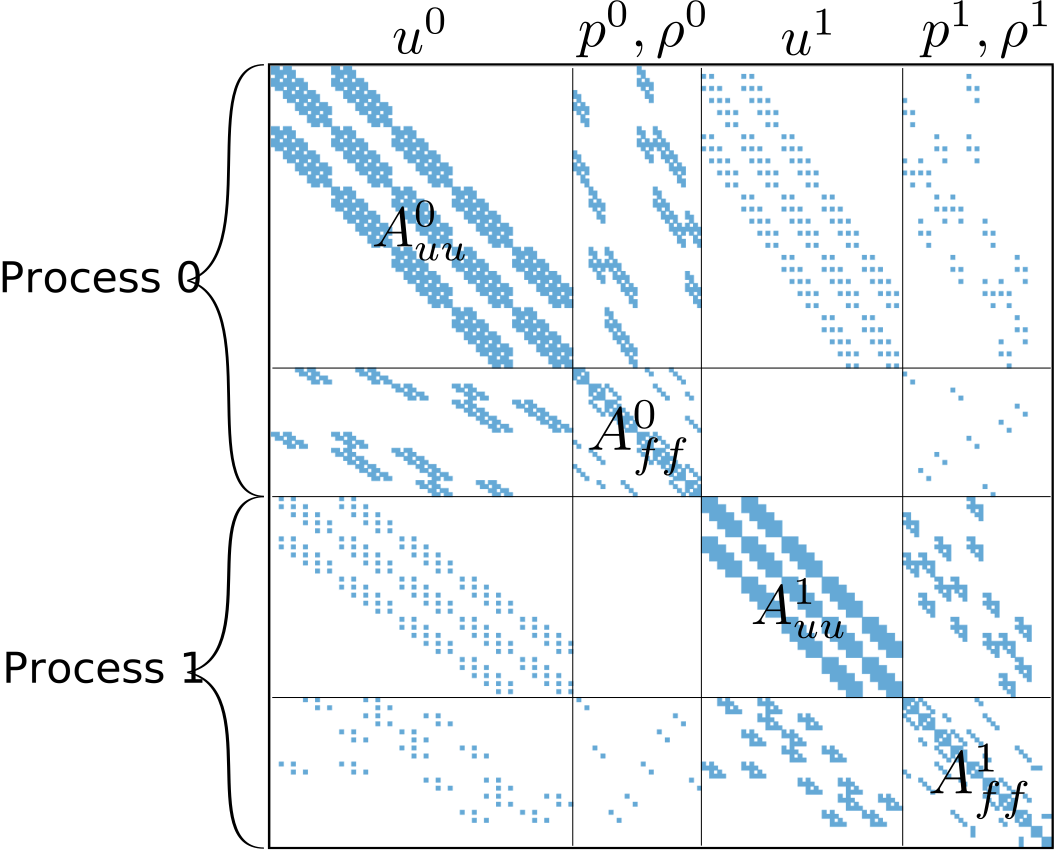
\includegraphics[width=0.5\linewidth]{figs/coupled_system_parallel_sparsity}}
  \caption[Sparsity pattern of a distributed multi-physics system matrix]{\label{fig:coupled_sparsity_parallel} Sparsity pattern of a fully-implicit coupled system matrix distributed over 2 parallel processes.   Degrees-of-freedom are ordered globally by process, while within each process displacement unknowns are enumerated first, followed by interleaved cell-centered flow (pressure) and transport (component density) unknowns.}
\end{figure}

We have developed a powerful \texttt{DofManager} component that abstracts away this complexity behind a set of simple interfaces for defining fields and coupling between them.   In addition to enumerating unknowns, we have implemented capabilities to construct matrix sparsity patterns for common coupling schemes (e.g. between low-order finite-volume and finite-element degrees-of-freedom), and to build restriction operators that can be used to extract and manipulate matrix/vector blocks of a larger ''monolithic'' system.   \texttt{DofManager} simplifies the development of both single-physics and coupled solvers as well as multiphysics preconditioning algorithms.

\subsubsection{Library Interfaces}

As explained in \cref{sec:intro_problem}, GEOSX must rely on fast and scalable linear solvers for its overall performance.   Developing general-purpose linear algebra libraries is an arduous effort that is usually undertaken by large groups of experts.   Examples of well established libraries in the numerical modeling community include \textit{hypre} \cite{hypre}, Trilinos \cite{trilinos-website} and PETSc \cite{petsc-user-ref}.   Rather than building the entire linear algebra infrastructure from scratch (unlikely to be a productive effort) or enforcing the use of a particular external library, we have taken the approach of defining a set of generic linear algebra \textit{interfaces} and implementing these interfaces for an open set of libraries that we refer to as \textit{backends}.   Currently our framework provides fully-implemented interfaces to the aforementioned three libraries, with the ability to define additional ones should a need arise.   For performance and compilation speed reasons, the backend used by all physics solvers must be selected at build configuration time.   However, should the user need to access capabilities of a different package, they only need to perform reconfiguration and partial rebuild of the simulator, without any code changes.

Every linear algebra interface must provide several key abstraction types that can be used to build more complex algorithms.   Each type encapsulates the data structures specific to the underlying backend library and invokes its API as needed.   If the needed functionality is not available directly in the library, we implement it in the abstraction type, either operating directly on the library's data structures if possible (and using RAJA to dispatch work in parallel), or building it out as a combination of library's existing APIs.   Each of the abstractions is interoperable only with other abstractions of the same backend, which is enforced through the type system.

\paragraph{Vector}
A general abstraction over a vector distributed across processes in a non-overlapping manner.   Provides high-level operations such as vector norms, scalar, dot and Hadamard products, scaling and linear combination (known as \texttt{axpy} in BLAS-1).   Since memory representation of the local part of a vector is simple (a single contiguous memory allocation) and generally the same across all libraries, we chose to explicitly manage vector's storage via our \texttt{Array} type and let backend APIs operate directly on it.   As a benefit, the rest of the framework can directly access vector's data in a safe and performant way in any memory space (by creating an \texttt{ArrayView} of it), so no copying is involved when assembling the residual vector or applying the linear system solution to update simulation state.

\paragraph{Matrix}
Similarly, an abstraction over a sparse matrix distributed by non-overlapping sets of rows.   Columns of the matrix are not physically distributed, but their logical ownership is also distributed across processors in a non-overlapping fashion.   Supported high-level operations include queries (computation of norms, extracting diagonal and row sums), modification (element, row or column scaling, element filtering, changing diagonal, transposition), matrix-vector operations (multiplication and transpose-multiplication) and matrix-matrix operations (multiplication, transpose-multiplication, triple product and its variations).   Unlike vectors, matrix implementations in different backends make different design choices about memory layout (for example, whether local and off-processor parts of the local rows are stored together or separately).   Therefore at present GEOSX lets different implementations manage their own memory, and provide (copy-based) interoperability with \texttt{CRSMatrix} objects which allows Jacobian assembly routines to remain independent of the selected backend and run in a correct and performant way in any execution space.
 
\paragraph{Preconditioner} 
Abstracts away the details of using various preconditioners available in external libraries.   The user is presented with a unified interface, allowing them to configure the preconditioning method through a common but extensible set of parameters, setup the preconditioner from a given matrix, and apply it to a given vector.   Under the hood, the implementation attempts as best as possible to match the selected option configuration to the capabilities of a particular library and dispatch to its APIs, passing to them unwrapped matrix and vector representations.

\paragraph{Solver}
Finally, a wrapper around external library solvers is provided by each interface, giving users access to more advanced iterative methods and optimized implementations (in addition to GEOSX's own backend-agnostic Krylov solvers), and allowing for potentially tighter integration between the iterative method and the preconditioner in a particular package.

\subsubsection{Block Preconditioner}

To facilitate the development of custom multi-level and multi-physics preconditioners, we have developed a flexible template for a $2 \times 2$ block preconditioner that is parametrized on the vector type and therefore works with any linear algebra backend.   The operator is implemented in a general form: given an arbitrary partitioning of a system matrix $A$ into blocks
\begin{align}
  A = P_\pi^T
  \begin{bmatrix}
      A_{11} & A_{12} \\
      A_{21} & A_{22}
  \end{bmatrix}
  P_\pi
  \label{eq:block_precond_part}
\end{align}
(with $P_\pi$ an optional permutation matrix that separates the blocks), action of the preconditioner is 
\begin{align}
  M^{-1} = P_\pi^T
  \underbrace{\begin{bmatrix}
  I_{1} & -M_{1}^{-1}A_{12} \\
        &  I_{2}
  \end{bmatrix}}_{\widetilde{U}^{-1}}
  \underbrace{\begin{bmatrix}
  M_{1}^{-1} &            \\
             & M_{2}^{-1}
  \end{bmatrix}}_{\widetilde{D}^{-1}}
  \underbrace{\begin{bmatrix}
   I_{1}            &       \\
  -A_{21}M_{1}^{-1} & I_{2}
  \end{bmatrix}}_{\widetilde{L}^{-1}}
  P_\pi
  \label{eq:block_precond}
\end{align}
where $M_1^{-1} \approx A_{11}^{-1}$, $M_2^{-1} \approx S_{22}^{-1}$ are arbitrary preconditioners for the sub-problems (e.g. multigrid solvers) and
\begin{align}
    S_{22} \approx A_{22} - A_{21} A_{11}^{-1} A_{12}
\end{align}
is a sparse Schur complement approximation that is computed in one of several ways described in \cref{subsec:coupled_smoothing}.   The user can control the type of Schur complement, the shape of the preconditioner (one or both of the $\widetilde{U}^{-1}$ or $\widetilde{L}^{-1}$ in \cref{eq:block_precond} can be disabled, resulting in a lower- or upper-triangular scheme), as well as any options for $M_1^{-1}$ and $M_2^{-1}$.   In particular, either of the two sub-block solvers can be another instance of block preconditioner, resulting in a multilevel reduction scheme that can be used to recursively tackle problems with 3 or more unknown types (similar to \textit{hypre}'s MGR solver \cite{Bui2020}, albeit with a slightly less efficient implementation and the lack of global smoothing option).   The partitioning into blocks \cref{eq:block_precond_part} is specified by the physics solvers that creates the preconditioner, in conjunction with \texttt{DofManager} that provides the needed reordering $P_\pi$.   Uses of block preconditioner in GEOSX include fixed-stress preconditioning for single-phase poromechanics \cite{White2015} and block smoothing for the coupled multiscale solver as described in \cref{subsec:coupled_smoothing}.

\subsubsection{Iterative Solvers}

We have implemented a suite of preconditioned iterative solvers in GEOSX, including a fixed-point modified Richardson scheme (useful for research purposes) and Krylov subspace solvers (CG, BiCGStab and GMRES).   Since each method is expressed entirely in terms of vector operations, each solver is only parametrized by the vector type and accepts the system matrix and preconditioner in the form of arbitrary objects implementing a simple \texttt{LinearOperator} interface.   This interface is implemented by all Matrix and Preconditioner types from library interfaces, but it can be easily satisfied by other user-defined types too.   One particular use of this capability are matrix-free methods that can reach a high computational throughput and reduced memory footprint on GPUs, especially for higher-order discretizations.   A matrix-free solid mechanics solver is currently under active development in GEOSX.   Another use of ''native'' iterative solvers (as opposed to external library implementations) is to allow for a fair comparison of custom preconditioners, such as the multiscale method that is the subject of present work, against state-of-the-art preconditioners in third-party libraries --- using the same solver code eliminates the potential differences in convergence and performance related to solver implementation details.

% ===================== SECTION =====================
\section{Summary}
\label{sec:geosx_summary}

In this chapter we presented the design and several key elements of the GEOSX multiphysics simulation framework.   The performance portability abstractions and efficient data containers described are foundational for the development of both accelerated physics solvers and advanced preconditioning algorithms within the framework.   